\documentclass[12pt]{article}
\usepackage{graphicx}
\usepackage{booktabs}
\usepackage[margin=1.0in]{geometry}
\usepackage{color}
\usepackage{tabularx}
%Times New Roman 12 pt
\usepackage[T1]{fontenc}
\usepackage{mathptmx}
\usepackage{amssymb}
\usepackage{amsmath}
\usepackage{authblk}
\usepackage[backend=bibtex,style=phys]{biblatex}

\graphicspath{{snapshots/}}

\newcommand{\angstrom}{\textup{\AA}}

\title{}
\author[1]{Lisa E. Felberg}
\author[2]{Luis A. Ruiz Pestana} 
\author[1-4]{Teresa Head-Gordon} 

\addbibresource{references}

\affil[1]{Department of Chemical and Biomolecular Engineering, University of California Berkeley, 
Berkeley, California 94720, USA}
\affil[2]{Chemical Sciences Division, Lawrence Berkeley National Labs
Berkeley, California 94720, USA}
\affil[3]{Department of Chemistry, University of California Berkeley, 
Berkeley, California 94720, USA}
\affil[4]{Department of Bioengineering, University of California Berkeley, 
Berkeley, California 94720, USA}


\date{}
\setcounter{Maxaffil}{0}
\renewcommand\Affilfont{\itshape\small}

\begin{document}
	\maketitle
\clearpage

\section*{Abstract}

\clearpage

\section*{Introduction}

The study of water in its many forms has always been an area of great interest for a range of scientific studies, due to its ubiquity and unique long-range structure and properties. In contrast to water in a bulk environment, water in a confined environment exhibits drastically different structural and dynamic properties. Although it may not immediately be apparent, water in a confined form is just as ubiquitous as that in bulk, from biological systems (cell interiors, and membrane pores and channels), as well as industrial systems (presence of moisture in instruments).  Thus, the characterization of water in confinement has recently become a growing field field with applications in a variety of domains, including biological applications \cite{Chaban2011,Schneider2010}, microfluidics \cite{Prakash2008} and energy conversion \cite{Dhiman2011,Siria2013}.

The introduction of hydrophobic walls immediately alters the structure of water by introducing anisotropy. Additionally, the form of these walls, e.g. in parallel walls or nanosized tubes, reduces the dimensionality of the system, to 2D and 1D, respectively. The effect of the hydrophobic confinement is generally analyzed by a characteristic length scale, such as plate separation for lamellar systems, and pore diameter for nanotubes. With larger length scales, the systems are typically divided into a core-shell or two-state model \cite{Korb1994, Liu1991}, which considers two different regions of confined water - those in the core are far enough from the wall that they behave like bulk water and those in the shell, whose properties are affected by the presence of the wall. Confined solute properties and experimental results can then be interpreted as a linear combination of these two regions. Recently  \cite{Laage2012}, the validity of this approximation has been examined, and it is also evident that this model is not valid at length scales commensurate with the size of water solvation shells. 

At the smaller length scales, all confined water is affected by the presence of an interface. Structurally at the smallest confinement lengths, water adapts ice-like structures, both in carbon nanotubes (CNT) and lamelllar graphene. In the carbon nanotubes, it has been seen that the ice monolayer mimics the cylindrical nature of the CNT, through x-ray diffraction and molecular dynamics (MD) studies \cite{Maniwa2005}. In graphene sheets, ice has been seen in transmission electron microscopy (TEM) \cite{Algara-Siller2015} as well as MD simulations of monolayers and bilayers of water \cite{Zangi2003,Zangi2003_2}.

Computational studies of confined water generally use a rigid model of graphene, but studies of isolated graphene sheets and other 2D nanomaterials reveal that these surfaces exhibit wrinkles and ripples  \cite{Fasolino2007, Los2009, Gao2014}. Mermin-Wagner theorem \cite{Mermin1968} states that long-wavelength fluctuations should destroy the order of 2D crystals, yet experiments have shown \cite{Meyer2007} that freely suspended graphene sheets do exist with high degrees of microscopic roughening (variations in the surface normal and out-of-plane deformations of up to 10 \r A).

The thermal basis for rippling is the anharmonic coupling between bending and stretching modes, whereas mechanical whereas mechanical factors, such as edges and impurities are other sources of rippling. Computational efforts have been made to characterize the rippling of the graphene with estimations of bending rigidity and stiffness parameters \cite{Wei2012}, graphene sheets have been characterized with the continuum medium theory and normal-normal correlation functions have been fit with power-laws \cite{Los2009}. The length of the ripples has been reported to be on the order of 80 \r A \cite{Fasolino2007, Los2009}, which is also important because of its commensurability with many simulation domain sizes.

Beyond characterizing intrinsic ripples and wrinkles in graphene, efforts have been made to report the temperature dependence of ripples (disappeared when systems heated to 450-600K, reappeared with cooling), create and manipulate these ripples (thermal induced compression) \cite{Bao2009}. Ripples also have applications in domains of graphene electronics (the sp\textsubscript{2}-to-sp\textsubscript{3} bandgap creation at selective locations), the enhanced diffusion of droplets on rippled sheets for enhanced, controlled nanoparticle transport \cite{Ma2016}. Wrinkled and crumpled graphene may have use in applications such as energy storage and strain sensing \cite{Deng2016}, cooling devices \cite{Warzoha2014} and pollutant adsorption and removal \cite{Wang2016}.

Understanding the nature of flexibility and rippling is important for the formation of graphene from graphite, where a single layer of graphene is removed using liquid as a media. During this process, a common issue is the reaggregation of graphene sheets, so dynamic interactions need to be better understood. To our knowledge, only one study \cite{Deshmukh2014} has explored the effect of graphene flexibility on confined water, and for their analysis, finite graphene sheets were used. Comparing rigid and flexible, finite graphene sheets in larger water boxes, they found that the systems behaved differently as a function of decreasing plate separation. For rigid sheets, there was a monotonic increase of local ordering of the confined water, whereas for the flexible graphene, the increase in ordering was non-monotonic. Differences  in water properties between rigid and flexible graphene models were most apparent at the smallest plate separation (8 \r A), and were observed in structural properties such as density profiles and radial distribution functions as well as dynamic observables such as mean square displacements and vibrational spectra. 


\clearpage

\section*{Methods}

\subsection*{Models}

For this study, simulations of systems with parallel graphene plates with
separations of 6 and 12 \r A respectively in the x-cartesian dimension.
Systems of two different sizes were used to explore periodic size effects, with graphene
plate separation held constant. The smaller systems had y-z dimensions of 46.2 by 48.5 \r A
and the large systems had dimensions of 121.8 by 118.8 \r A.

\textbf{\color{red} How were they built?? }

\subsection*{Force fields}

Harmonic bond and angle potentials were applied to the graphene sheets with 
the following parameters: k\textsubscript{bond} = 938.0 \(kCal/mol/\angstrom^2\)
and k\textsubscript{angle} = 126.0 \(kCal/mol/rad^2\), equilibrium bond and 
angle lengths of 1.40 \r A and 120.0 degrees respectively \cite{Hummer2001}. The
dihedral potential is harmonic with the functional form: \(E_{\text{di}} = K_{\text{di}} [ 1 + d cos(\phi)]\),
where K\textsubscript{di} = 3.15 kCal/mol, \(\phi = 180.0\) degrees and \(d = \pm 1\) \cite{Patra2009}. An improper torsional 
potential with a harmonic functional form as follows: \( E_{\text{im}} = K_{\text{im}} [ \chi - \chi_0 ]^2\) was
used with parameters K\textsubscript{im} =  15.0 kCal/mol and \(\chi_0 = 0.0\) degrees. A summary
of these potentials and their parameter values are given in Table \ref{table:ff_parms}
The water model chosen is TIP4P-Ew \cite{Horn2004} was used 
to represent explicit solvent. Partial charges and Van der Waals parameters for each atom type 
are given in Table \ref{table:ff_parms_atoms}.

\begin{table}[ht!]
\centering
\begin{tabular}{ lllll } \hline
Bond     &         & \(K_b\)  (\(kCal/mol/\angstrom^2\))      & b\textsubscript{0}  (\r A)            &          \\ \hline
         & C-C     & 938.0         & 1.40            &          \\
         &         &               &                 &          \\ \hline
Angle    &         & \(K_{\theta}\)  (\(kCal/mol/rad^2\)) & \(\theta_0\) (degrees)   &          \\ \hline
         & C-C-C   & 126.0         & 120.0           &          \\
                           &         &               &                 &          \\ \hline
Improper &         & K\textsubscript{im} (kCal/mol)       & \(\chi_0\) (degrees)     &          \\ \hline
         & C-C-C-C & 15.0          & 0.0             &          \\
                           &         &               &                 &          \\ \hline
Dihedral &         & K\textsubscript{di} (kCal/mol)       & n (multiplicity) & \(\phi\) (degrees)\\ \hline
         & C-C-C-C & 3.150         & 2               & 180.0  \\ 
\end{tabular}
\caption{\textit{Force field bonded parameters used for graphene in confined water simulations.}}
\label{table:ff_parms}
\end{table}

\begin{table}[ht!]
\centering
\begin{tabular}{|c|r|r|r|}
\hline
\textbf{Atom type} & \multicolumn{1}{c|}{\textbf{\begin{tabular}[c]{@{}c@{}}Partial charge\\ (e)\end{tabular}}} & \multicolumn{1}{c|}{\textbf{\begin{tabular}[c]{@{}c@{}}Sigma\\ (\r A)\end{tabular}}} & \multicolumn{1}{c|}{\textbf{\begin{tabular}[c]{@{}c@{}}Epsilon\\ (kCal/mole)\end{tabular}}} \\ \hline
Graphene carbon    & 0.0000                                                                                     & 3.55000                                                                              & 0.07000                                                                                     \\ \hline
Water oxygen       & -1.0484                                                                                    & 3.16435                                                                              & 0.16275                                                                                     \\ \hline
Water hydrogen     & 0.5242                                                                                     & 0.00000                                                                              & 0.00000                                                                                     \\ \hline
\end{tabular}
\caption{\textit{Force field parameters used for each atom type in confined water simulations.}}
\label{table:ff_parms_atoms}
\end{table}


\subsection*{Simulation protocols}

Simulations were performed with the LAMMPS software package \cite{Plimpton1995}. 
Equilibration of initial configurations were performed as follows. Systems were run in 
the NVE ensemble with a Langevin Thermostat at 298 Kelvin
for 10 ps. The water was then fixed with the SHAKE protocol \cite{Andersen1983} with a tolerance
of 10\textsuperscript{-4} and the system was run for 10 ps in the NVT ensemble.
Finally, data was saved for analysis in a production run in the NpT ensemble,
during which all cartesian coordinates were stored every 500 timesteps. 
Systems were run in the NpT ensemble for 10 ns. The 
pressure in the direction orthogonal to the graphene walls was maintained at 1 atm.
Thermal and pressure control were implemented using a Nos\' e-Hoover 
extended Lagrangian procedure \cite{Martyna1994} with characteristic damping times of 100 
and 1000 fs (0.1 and 1.0 ps), respectively. The dynamical integration 
scheme was velocity-Verlet \cite{Swope1982}.
For all simulations, the dynamics timestep was set at 2.0 femtoseconds. 

\subsection*{Analysis}

\begin{figure}[h!]
	\centering
	(a)~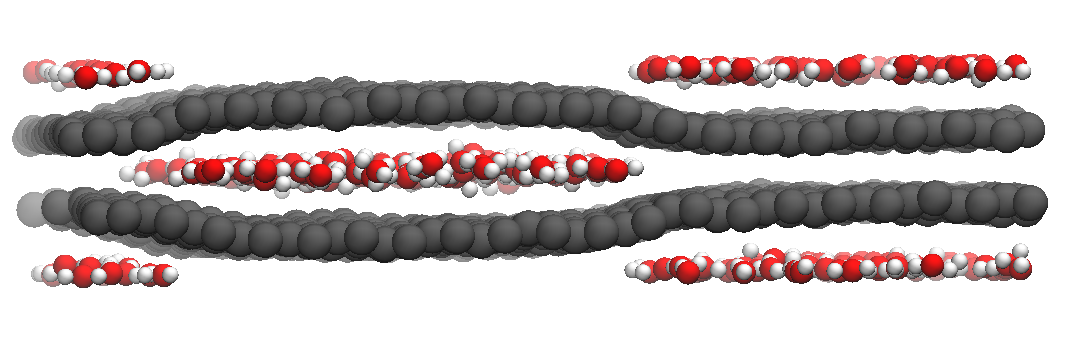
\includegraphics[width=0.45\linewidth]{d6L46_side} 
	(b)~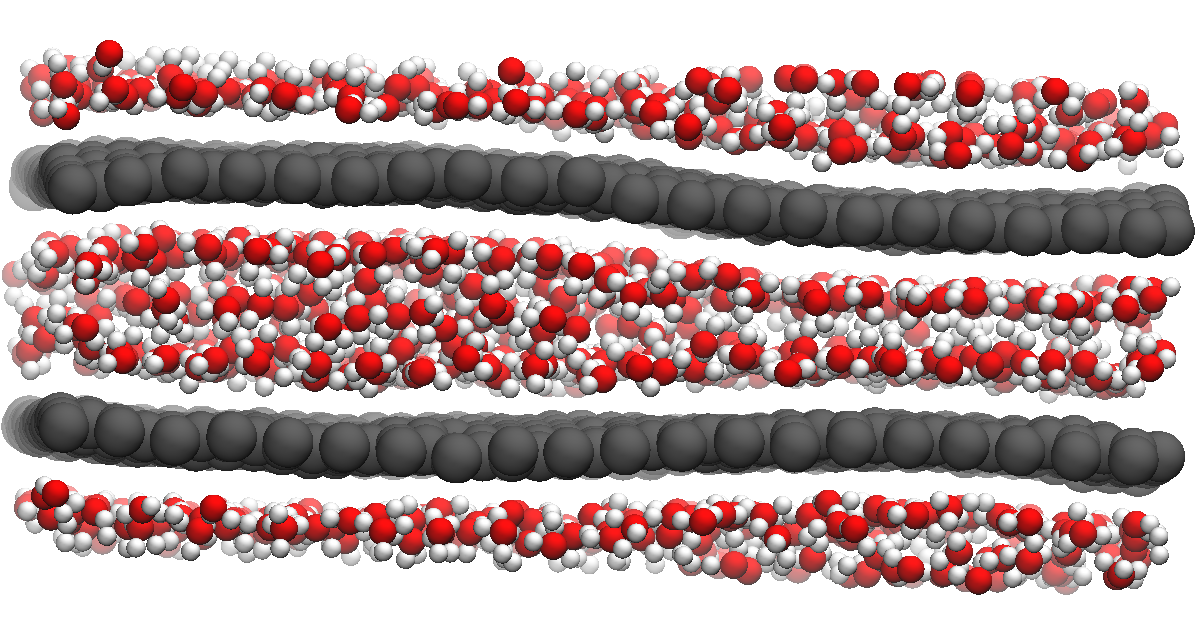
\includegraphics[width=0.40\linewidth]{d12L46_side}
	\vspace{-10pt}
	\caption{\textit{Snapshots of flexible confined systems.} Graphene carbons in grey, water oxygens in red and water hydrogens in white. (a) 6 \r A separated system (b) 12 \r A separated system. }
	\label{fig:chem_forms}
\end{figure}




\clearpage
\printbibliography
\end{document}

\clearpage

%%%%%% Intro notes

%Significance: many simulations have been performed with rigid graphene models, but if they are flexible, they may interact with the water in in different ways. \\
%
%\begin{itemize}
%\item General statement about studying water, the importance of water for various applications
%\item Difference of water in confined systems vs bulk
%	\begin{itemize}
%    		\item Difference of structure in confinement
%			\begin{itemize}
%				\item Anisotropy of the system, due to the presence of an interface
%				\item Reduction of dimensionality of water - 2D for lamella, 1D for cylindrical pore.
%                        		\item Enhanced ordering of the water near the interface
%				\item Larger distances - core/shell models
%                        		\item Transition from liquid-like to solid-like water with small enough length scales
%                    	\end{itemize}
%    		\item Difference of dynamics in confinement (\textit{might not be used if not discussed in the paper}).
%	\end{itemize}
%\item Studies on graphene flexibility.
%	\begin{itemize}
%		\item Isolated graphene
%		\item Graphene + water
%	\end{itemize}
%\end{itemize}

Dynamic properties: viscosity, velocity correlation functions, hydrogen bond reorientation

Things that could be varied:

1. The shape of confinement: lamella, cylinders, pores
2. The nature of the confinement: hydrophobic, hydrophilic, charged, uncharged
3. The length scales of confinement: size confiner - pore diameter, lamella separation

\subsection*{Previous studies on confined water:}

1. Water in rigid graphene

2. Water in flexible graphene - used finite graphene sheets, did 

Deshmukh et al (2014) performed classical MD of finite graphene sheets in water boxes. 

\subsection*{Citations}

\cite{Maniwa2005} 2005, XRD and MD studies of CNTs with varying diameters (10.9 - 15.2 \r A). Found four different structures. 
Also the melting temperature of the ice changed as a function of CNT diameter.


\cite{Algara-Siller2015} 2015, TEM and MD of ice in between graphene monolayers - saw ice of 1, 2 and 3 monolayers (with TEM).
With MD (SPC/E water), graph sheets of 68X58 \r A, and separations of 6.5, 9.0 11.5 \r A. ** VDW pressure, for a cluster of water between
two sheets??

\cite{Zangi2003,Zangi2003_2} 2003, studies of freezing and melting water of monolayer and bilayer ice.



%% BENZENE STUFF

%The benzene parameters were taken from the OPLS-AA force field \cite{Jorgensen1996}.
%The atom type \#145 was used for benzene carbons and \#146 was used for benzene
%hydrogens. This is from the papers: J. Am. Chem. SOC. 1990, 112, 4168-4114 \cite{Jorgensen1990}.
%and J. Am. Chem. Soc. 1996, 118, 11225-11236  \cite{Jorgensen1996}.  
%
%Nonbonded parameters
%\#   AN AT   CHARGE     SIGMA    EPSILON 
%145 06 CA   -0.115     3.550     0.070     Benzene C - 12 site JACS,112,4768-90
%146 01 HA    0.115     2.420     0.030     Benzene H - 12 site  "
%
%For bonds and angles, the following parameters were taken from AMBER all-atom
%\cite{Weiner1986} (also from zarbi.chem.yale.edu/doc/par\_opls\_aam.inp)
%Which has different CA-HA, and angle params.
%
%Bonds
%CA-CA 469.       1.40         TRP,TYR,PHE
%CA-HA 367.       1.080        PHE, etc. 
%
%Angles
%CA-CA-CA    63.        120.     PHE(OL)
%CA-CA-HA     35.       120.
%
%
%Torsions
%\#      v1        v2        v3       v4         notes
%165   0.0       7.250     0.0       0.0        CA-CA-CA-CA                           
%
%Improper
%improper\_coeff 1 1.1 -1 1  \# CA-CA-CA-HA for benzene 







